\chapter[Experimentos y resultados]{Experimentos y resultados}\label{ch:capitulo5}
En este capítulo presentaremos los experimentos y resultados obtenidos para la primera parte de este trabajo, el objetivo de este capítulo es discutir los resultados entregados por el framework presentado en el Capítulo~\ref{ch:capitulo4} con el fin de mostrar su rendimiento para las distintas clases utilizadas. Con esto obtendremos una visión detallada del funcionamiento de los modelos.

\section{Base experimental}
Para esta primera etapa se utilizó el framework presentado en el Capítulo~\ref{ch:capitulo4}, con éste se crearon modelos para distintas clases de objetos, botellas, personas, autos, sillas, etc. El sistema mostrado en el Capítulo~\ref{ch:capitulo4} a sido evaluado con las imágenes de prueba pertenecientes al conjunto de datos PASCAL VOC, conjunto de datos muy utilizado por otras investigaciones y que proporciona un sistema de anotaciones ideal para este tipo de trabajos. 

Cada conjunto de datos contiene miles de imágenes que representan objetos del mundo real, y  donde se especifican la posición del objeto por medio de cuadros delimitadores, además de registrarse información de la clases a la cual pertenece, entre otros datos. En la fase de pruebas, el objetivo es predecir la ubicación del cuadro delimitador de todos los objetos según la clases que se esté observando. En la practica, el sistema entrega como respuesta un conjunto de cajas delimitadoras con una puntuación de confianza, estas puntuaciones son delimitadas por un umbral en distintos puntos, lo que permite obtener una curva de precisión-exhaustividad, más conocido como \textit{precision}-\textit{recall}, a través de todas las imágenes de prueba. Para un umbral en particular, la precisión es la fracción de los cuadros delimitadores que entregan una correcta detección, mientras que la exhustividad (\textit{recall}), es la fracción de objetos encontrados.

Un cuadro delimitador es considerado correcto si este tiene al menos un 50\% de su tamaño contenido dentro del cuadro delimitador real. En caso de que varios cuadros delimitadores coincidan con el cuadro delimitador real, solo se deja uno como correcto. Por cada uno de estos cuadros se calcula un \textit{score} el que discrimina cual cuadro es mejor de acuerdo a su posición.

\section{Resultados}
En esta sección presentamos los resultados obtenidos para la detección de objetos. Con la ayuda del framework se creó un modelo de reconocimiento para botellas, autos, personas y bicicletas, luego se seleccionó un conjunto de imágenes para utilizar como datos de prueba, La Figura~\ref{fig:clases} muestra un extracto de algunas imágenes utilizadas para las distintas clases, con esto comprobamos la efectividad del modelo. Los resultados por cada clase se presentan la sección~\ref{sec:results}.
\begin{figure}[tb]
\centering
 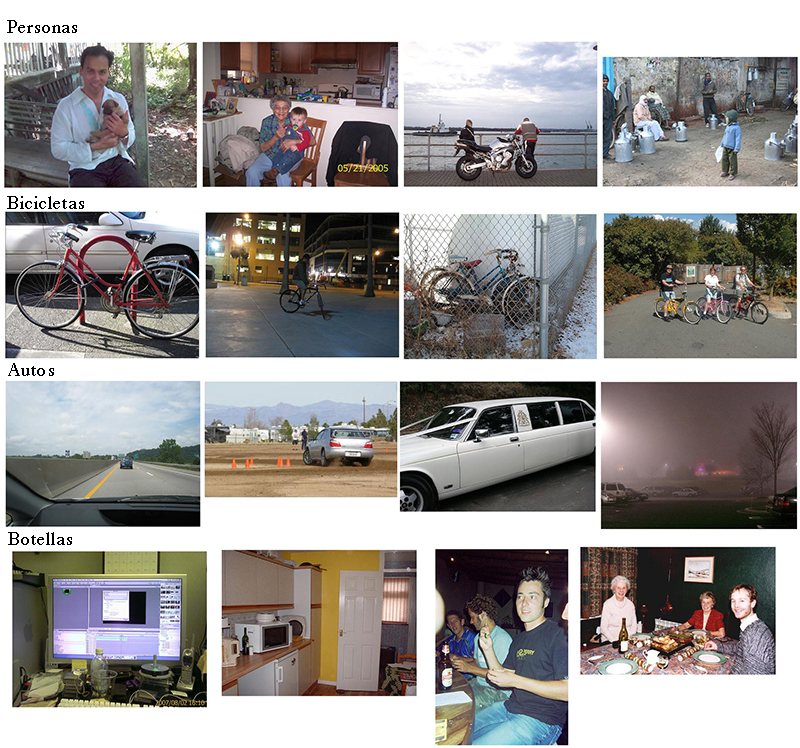
\includegraphics[width=1\textwidth]{Figuras/results/clases.jpg}
 \caption[Imágenes de prueba]{Imágenes de prueba para cada categoría,}
 \label{fig:clases}
\end{figure}
\section{Resultados experimentales}\label{sec:results}
En esta sección presentamos los resultados obtenidos por los modelos creado mediante la utilización del framework presentado en el Capítulo~\ref{ch:capitulo4}.

\begin{figure}[tb]
\centering
 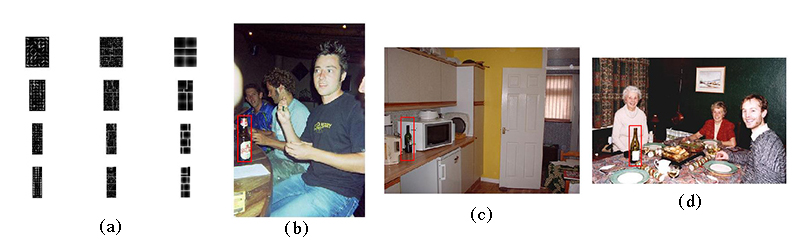
\includegraphics[width=1\textwidth]{Figuras/results/bottle_r/resultados.jpg}
 \caption[Detección de partes para un objeto (botellas)]{Resultados detección de botellas, en esta figura se muestran las partes obtenidas por el modelo creado por el framework (a), además se observan algunas imágenes con sus respectivas detecciones (b), (c) y (d). En este caso se trata de un modelo de detección de botellas.}
 \label{fig:botellas}
\end{figure}

\begin{figure}[tb]
\centering
 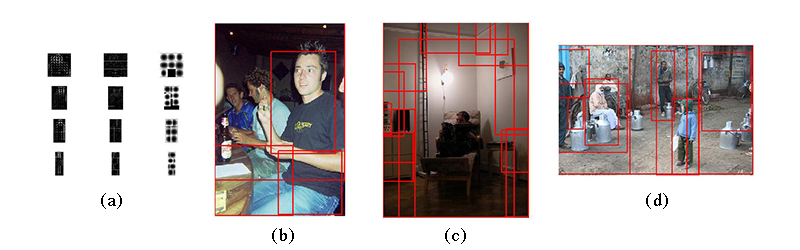
\includegraphics[width=1\textwidth]{Figuras/results/person_r/resultados.jpg}
 \caption[Detección de partes para un objeto (personas)]{Resultado de detección de personas, (a) muestra el modelo generado por el framework, en (b), (c) y (d) se muestran los resultados obtenidos en la detección por partes.}
 \label{fig:personas}
\end{figure}

\begin{figure}[tb]
\centering
 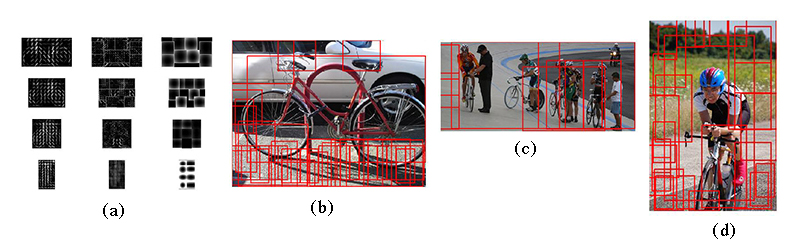
\includegraphics[width=1\textwidth]{Figuras/results/bicycle_r/resultados.jpg}
 \caption[Detección de partes para un objeto (bicicleta)]{Resultado detección de bicicletas, (a) muestra el modelo generado por el framework, en (b), (c) y (d) se muestran los resultados obtenidos en la detección por partes.}
 \label{fig:bicicleta}
\end{figure}

Si bien en las tres clases mostradas como ejemplo se obtuvo un modelo de predicción, algunos modelos son mejores que otros, y en este caso si nos detenemos en la Figura~\ref{fig:botellas}, podemos darnos cuenta que no tiene ruido al detectar un objeto, entiendase por ruido a la presencia de otras regiones delimitadoras, a diferencia de las Figuras~\ref{fig:bicicleta} y~\ref{fig:personas} que presentan mucho ruido. Esto es debido a que estás dos últimas clases (bicicletas y personas) han sido deliberadamente entrenadas con una menor cantidad de ejemplo, influyendo notoriamente sobre los resultados obtenidos. A su vez la cantidad de iteraciones sobre un mismo ejemplo se redujo con el objetivo de disminuir el tiempo de computo, obteniendo como resultado un peor predicción. Para el caso del modelo de botellas este tuvo una duración de 8 horas, donde no se limito el número de datos de entrenamiento, siendo este de 5813 imágenes. Además sobre cada ejemplo se iteró, para ejemplos positivos 10 veces y para ejemplos negativos 8 veces, logrando así una mejora sustancia sobre el modelo de predicción.

\subsection{Modelos para expresiones faciales}\label{subsec:m_face}
Para las expresiones faciales, se separaron estas expresiones en seis clases, correspondientes cada una de ellas a las expresiones canónicas, es decir, obtuvimos un conjunto de imágenes de entrenamiento para expresiones de alegría, asco, ira, miedo, sorpresa, tristeza. El objetivo es generar un modelo de predicción para cada una de estas expresiones. Si bien no se generó un modelo final para estás expresiones, ya que se dio mayor énfasis en el análisis del framework y los modelos para objetos. 

\section{Resumen}
En este capítulo se presentaron los experimentos realizados en esta etapa y algunos resultados obtenidos correspondientes al funcionamiento del marco de desarrollo descrito en el Capítulo~\ref{ch:capitulo4}. Podemos apreciar en la Figura~\ref{fig:botellas} que la detección de un objetos del tipo botella, ha sido posible mediante la creación de un modelo creado mediante la utilización de muchos datos de entrada que tenían precian de una botella, como se mencionó anteriormente estos datos son proporcionados por la base de imágenes de PASCAL. En el siguiente capítulo se presentan nuestras conclusiones sobre esta primera etapa del trabajo, además se presentan los trabajos pendiente y futuros que se realizarán en futuras entregas.


